%! Author = User
%! Date = 13.09.2023

% Preamble
\documentclass[a4paper,10pt,twocolumn]{article}

% Packages 
\usepackage[utf8]{inputenc}  %man kann Sonderzeiche wie ü,ö usw direkt eingeben
\usepackage{amsmath}           %macht
\usepackage{amsfonts}          %       Mathe
\usepackage{amssymb}           %              mächtiger
\usepackage{graphicx}          %erlaubt Graphiken einzubinden (.eps für dvi und ps sowie .jpg für pdf)
\usepackage[T1]{fontenc}       %Zeichenbelegung der verwendeten Schrift
\usepackage{ae}                %macht schöneres ß
\usepackage{typearea}
\usepackage{amstex}
\usepackage{siunitx}
\usepackage{hyperref}	         %ermöglicht änderung des Seitenspiegels
\usepackage{subcaption}


\usepackage{amsmath}
\usepackage{tikz}
\usepackage{pgfplots}

\newcommand{\alphaNoError}{(4.047 \pm 0.036)}
\newcommand{\betaNoError}{(-4.73 \pm 0.29) \cdot 10^{-3}}
\newcommand{\halfTimeNoError}{(146.5 \pm 9.1)\ s}
\newcommand{\alphaGauss}{(4.04 \pm 0.10)}
\newcommand{\betaGauss}{(-4.62 \pm 0.95) \cdot 10^{-3}}
\newcommand{\halfTimeGauss}{(150 \pm 31)\ s}
\newcommand{\alphaPoisson}{(4.05 \pm 0.10)}
\newcommand{\betaPoisson}{(-4.75 \pm 0.95) \cdot 10^{-3}}
\newcommand{\halfTimePoisson}{(146 \pm 29)\ s}
\newcommand{\symN}{\delta N}



\pagestyle{scrheadings}        %sagt Koma-Skript, dass selbstdefiniers Kopfzeilen verwendet werden
\typearea{16}                  %stellt Seitenspiegel ein
\columnsep25pt								 %definiert Breite zwischen den zwei Spalten von \twocolumns

\renewcommand{\pnumfont}{%     %ändert die Schriftart der Seitennummerierung
    \normalfont\rmfamily\slshape}  %ändert die Schriftart der Seitennummerierung 



\begin{document}
    \twocolumn[{\csname @twocolumnfalse\endcsname                %erlaubt "Abstrakt" über beide Spalten
    \titlehead{                                                  %Kopfzeile
        \begin{tabular*}{\textwidth}[]{@{\extracolsep{\fill}}lr}   %Kopfzeile
            Tutor: Jochen Kaupp & \today\\                          %Kopfzeile - Betreuer
        \end{tabular*}                                             %Kopfzeile
    }
    \title{Experimental methods for examining properties of classical light with microwaves: Polarisation, Total Reflaction
    and tunneling; Using crystal model to demonstrate bragg reflection}  %Titel der Versuchs
    \author{Salahudin Smailagić and Thomas Karb}                     %Namen der Studenten
    \date{}                                                         %benötigt um automatisches Datum auszuschalten
    \maketitle                                                      %erzeugt Titelseite
    \vspace{-5ex}                                                   %verringert Abstand zur Überschrift
    \begin{abstract}                                                %Beginn des Abstracts
%        We use microwaves to study the wave character of light.
%        Thier wavelength in cm range make it possible to reveil properties of EM-waves, which would
%        for visible light require significantly more complex setups.
%        Firstly the wavelength can be easely measured by counting nodes.
%        Herefor we use a setup with standing waves and a michelson interferometer.
%        We verify polarisation and Malus'law for linear-polarisation-filters.
%        Furthermore we show total reflection and the tunnel effect, which only can be explained
%        by the wave character of the used microwaves.
%        These effects are then applied for bragg diffraction.
%        We use an exemplary crystal model to demonstrate the principle.
%        At last we show qualitatively the usage of a metal tube as waveguide.
        
        Die Maxwell-Gleichungen beschreiben Licht als elektromagnetische Welle.
        Ziel dieses Papers ist der Nachweis der Welleneigenschaften.
        Wir nutzen hierzu eine Gunn-Diode, welche Microwellen emittiert.
        Aus der Wellenoptik ergibt sich, dass vor einem Spiegel sich stehende Wellen ausbilden.
        Wir nutzen diese Eigenschaft, um die Wellenlänge der Diode zu bestimmen, indem wir die Knoten der sthenden
        Welle zählen: $\lambda = \StandingWavesWaveLength$.
        Ferner interferieren zwei überlagerte Lichtstrahlen.
        Mit Hilfe eines Micealson-Interferometers nutzen wir dies, für eine zweite Bestimmung der Wellenlänge 
        $\lambda = \InterferometerWaveLength$.
        Elektro-magnetische Wellen sind keine skalaren Wellen, sondern sind polarisiert.
        Dies weisen wir nach, indem wir einen linearen Polfilter verwenden.
        Wir können das Gesetz von Malus, welches die Durchlass-Intensität des Polfilters in Abhängigkeit des Winkels
        beschreibt, zu mindest qualitativ bestätigen.
        Hinter einer Fläche, an der die Lichtstrahlen totalreflektiert werden, bildet sich laut der Theorie
        evaleszente Wellen aus. % TODO Rechtschreibung
        Wir weisen diese nach unter Verwendung zweier Wachsprismen.
        Die Intensität der evaleszenten Welle nimmt exponentiell ab, was wir bestätigen können.
        Die Reflexions- und Interferenzeigenschaften macht sich die Methode der Bragg-Reflexion zu nutze,
        um Gitterkonstanten zu bestimmen.
        Wir demonstrieren das Prinzip anhand eines Kristallmodels.
        Zu letzt zeigen wir qualitativ, dass ein Metalschlauch als Wellenleiter verwendet werden kann.
        
        \\
        Measuerement made: 21. September 2023\\       %Datum ändern!
        Submitted: 28. September 2023                %Datum ändern!
        \\
        \\
    \end{abstract}
    }] 
    \section{Introduction}
    To study wave-properties of light we use microwaves.
    They have a large wavelength in the cm-range.
    Effects like interference and tunneling occur on a macroscopic scale, which makes it easy to show them
    in an experiment.
    Because all properties shown here apply also for light in the visible spectrum, you can 
    adopt the presented methods on a smaller lengthscale.
    
    \section{Experimenteller Aufbau}
    Für unsere Experimente benutzen wir das `PASCO Microwave Optics System WA-9316A'.
    \subsection{Empfänger}
    
    Wir benutzten den im `PASCO'-System enthaltenen Empfänger ´WA-9802'.
    Er ist eine Scotty-Diode, welche nur linear polarisiertes Licht detektiert.
    Zur Fokussierung ist eine Horn-Antenne auf dem Empfänger montiert.
    Der Empfänger gibt eine Spannung aus, welche wir dann mit dem Voltmeter Agilent 34405A messen.
    Es ist anzumerken die ausgegebene Spannung ist weder proportional zur Intensität $I$ der Mikrowellen oder zum E-Feld $E$.
    Stattdessen ist es ein Zwischenwert~\cite{pasco}.
    Aus diesem Grund können wir nicht von der Spannung auf die Intensität zurück rechnen.
    Deswegen sind in all unseren Daten nur die gemessenen Spannungen angegeben.
    Ferner gibt der Empfänger eine Spannung aus, auch wenn keine Mikrowellen vorhanden sind.
    Diese Nullpunktverschiebung ist aus den angegebenen Daten korrigiert worden.
    
    Für den Fehler ist in unseren Daten nur der Spannungsfehler des Voltmeters angegeben.
    Der Fehler der Diode kann nicht abgeschätzt werden.
    Da aber nicht von der Spannung auf die Intensität zurück gerechnet werden kann, sind alle 
    Messungen, welche die Intensität benötigen, nur qualitative Messungen.
    
    \subsection{Transmitter}

%    \figAngleDispersion{Angle dispersion of the Gunn diode used in our setup.
%    We fit a gauss curve to get an approximation of the variance.
%        $fwhm = \AngleDispersionGaussFWHM$}
    \figAngleDispersion{
        Die Winkeldispersion der in unserem Aufbau verwendeten Gunn-Diode.
        Der Empfänger wurde um denn Emitter geschwängt, und abhängig vom Winkel die Intensität zu messen.
        Wir passen eine generische Gaußkurve and die Daten an, um eine grobe Abschätzung der Streubreite zu erhalten:
        $fwhm = \AngleDispersionGaussFWHM$ . % TODO Graphiken
    }
    

%    A Gunn diode was used to create the microwaves in our experiments. 
%    It has a horn antenna for focusing the light.
%    We measured the angle-intensity-relation and made a basic gauss-fit to get a rough estimate of the light dispersion (cf.~\ref{fig:AngleDispersion}).
%    The full-width-half-maximum of the used emitter is

    Wir benutzen den Transmitter `WA-9801' aus dem `PASCO'-System.
    Dieser ist eine Gunn-Diode auf der ebenfalls eine Horn-Antenne montiert ist.
    Diese emittiert Mikrowellen mit einer Wellenlänge von $\lambda = \OfficialWaveLength$ laut Hersteller.
    
    Zu nächst wollen wir die Winkeldispersion der Gunn-Diode bestimmen, um etwaige Fehler durch eine
    große Streuung abschätzen zu können.
    In einem Bereich von $\pm 90 ^{\circ}$ messen wir die Intensität in Abhängigkeit des Winkels.
    Die Daten sind in Abbildung~\ref{fig:AngleDispersion} aufgetragen.
    Wir führen einen Gauß-Fit durch, um eine grobe Abschätzung der Lichtstreuung zu erhalten.
    Auf den tatsächlichen funktionellen Zusammenhang können wir nicht zurück schließen, da die gemessene Spannung
    nicht proportional zur Intensität ist.
    Das Full-width-half-maximum der verwendeten Diode ist
    
    \begin{align*}
        fwhm = \AngleDispersionGaussFWHM
    \end{align*}
    
    Der angegebene Fehler wurde über die Parameterfehlern des Fits bestimmt.
    Er bestimmt sich aus der Streuung der Datenpunkte.
    Der systematische Fehler, welcher sich aus der auf Grund der unbekannten Spannung-Intensität-Beziehung ergibt, kann
    nicht abgeschätzt werden.
    
    \subsection{Linse}

%    \figimageDistance{We measure the signal depending on the reciever-lens distance $b$.
%    The intensity fluctuates since a stationary wave overlaps.
%    We apply a gauss-fit to get the maximum image distance.
%    This can be used to calculate the focal length after the lens formula ~\eqref{eq:LensFormula}}
    \figimageDistance{Wir messen die Intesität in Abhängigkeit der Bildweite $b$.
    Die Intesität schwankt stark, da sich eine stehende Welle überlagert.
    Wir verwenden eine generische Gauß-Anpassung, um eine Abschätzung des Maximums zu erhalten:
    $b = \ImageDistance$.
    Mit der Abbildungsgleichung~\ref{eq:LensFormula} kann die Brennweite bestimmt werden:
    $f = \FocalLength$.
    }
    
%    For the experiments with bragg diffraction and tunnel effect we need parallel light rays.
%    We used a wax lens for focusing the emitted microwaves.
%    To determine the focal length, the lens was placed away from the emitting diode.
%    The object-distance\footnote{emitter-lense distance after ~\cite{pasco}} in our setup was $g = \ObjectDistance$
%    Then by varying the receiver positions the intensity was measured as shown in figure ~\ref{fig:imageDistance}. 
%    Because the wavelength is in the cm range, the diameter of the resulting airy disk is also in the cm range.
%    This means there is no distance were the object (emitter) is completely focused as you would expect from geometric optics.
%    So to get the actual image-distance you need to find the maximum.
%    Since we have few data points with much noise we use a gauss curve to find an approximation of the maximum.
%    Though the actual theoretical intensity-distribution is more complicated.

    Für die Experimente mit Bragg-Beugung und Tunneleffekt benötigen wir parallele Lichtstrahlen. 
    Wir verwendeten eine Wachslinse zur Fokussierung der emittierten Mikrowellen. 
    Um die Brennweite zu bestimmen, wird die Linse ca.\ $80 \mathrm{cm}$ entfernt von der emittierenden Diode platziert. 
    Die Gegenstandweite zwischen Linse und Transmitter betrug in unserem Aufbau $g = \ObjectDistance$.
    Hier zu wurde der Abstand zwischen der Mitte der Linse und der effektiven Position des Senders nach~\cite{pasco} gemessen.
    
    Nun wird der Empfänger auf der anderen Seite positioniert.
    Für verschiedene Abstände zur Linse wir die Intensität gemessen.
    Es muss auch hier die effektive Position des Empfängers nach~\cite{pasco} berücksichtigt werden.
    Der Intensitätsverlauf ist in Abbildung~\ref{fig:imageDistance} dargestellt.
    
    Da die Wellenlänge der Mikrowellen im cm-Bereich liegt, liegt auch der Durchmesser 
    des resultierenden Airy-Scheibchens hinter der Linse auch im cm-Bereich.
    Das bedeutet, dass es keine Entfernung gibt, in der das Objekt vollständig fokussiert ist, wie man es in der
    geometrischen Optik erwarten würde. 
    Um die tatsächliche Bildentfernung zu ermitteln, muss man also das Maximum finden.
    
    Wir verwenden auch hier wieder eine generische Gauss-Kurve, um dass Maximum abzuschätzen.
    Denn neben der oben beschrieben Verzerrung der Daten durch die Scotty-Diode, ist in dieser Messung ein
    starkes Rauschen vorhanden.
    Hinter der Linse bildet sich eine stehende Welle aus, welche den Verlauf überlagert.
    
%    Here the image distance is 
    
    Die über den Fit bestimmte Bildweite beträgt:
    
    \begin{align*}
        b = \ImageDistance
    \end{align*}

    Auch hier ist der Fehler aus der statistischen Streuung der Datenpunkte um den Fit bestimmt worden.
    Er spiegelt nicht die systematischen Fehler wieder.
%    Now we can calculate the focal length after the lens formula
    Mit der Bildweite können wir nun die Brennweite berechnen nach der Abbildungsgleichung:
    
    \begin{align}
        \label{eq:LensFormula}
        \frac{1}{f} = \frac{1}{b} + \frac{1}{g}
    \end{align}
%    We have determined the focal length of the lens in our setup as:
    Die Brennweite der von uns genutzten Linse ist:
    \begin{align*}
        f = \FocalLength
    \end{align*}
    
    \section{Wellenlängen Messung}
    \subsection{Stehende Welle}
%    For the first approach we create stationary waves.
%    We position a mirror opposite of the emitter in a distance of $1m$.
%    Then we move the receiver between mirror and diode and count the nodes of the resulting standing wave.
%    We then measure the distance around 40 nodes and can calculate the wavelength:
    
    Eines der grundlegendsten Phänomene, welches aus der Welleneigenschaft des Lichts folgt, ist das der stehenden Welle.
    Betrachten wir eine Eingangswelle.
    Diese wird reflektiert von einem Spiegel.
    Dann überlagern sich die Eingangs- und reflektierte Welle.
    Es bildet sich eine stehende Welle aus.
    Diese hat ortsfeste Minima bzw. \ Maxima der Intensität.
    
    In unserem Experiment erzeugen wir die stehende Welle, indem wir in einem Abstand von $1\, \mathrm{m}$ entfernt
    vom Transmitter einen Metalspiegel positionieren.
    Zwischen Transmitter und Spiegel entsteht dann eine stehende Welle.
    Diese messen wir mit dem Empfänger, aber ohne Horn-Antenne.
    Sie würde mit dem Signal interferieren.
    Wir variieren die Positions des Empfängers bis wir ein Minima gefunden haben.
    Nun verschieben wir ihn langsam und zählen wie viele Knoten wir durchlaufen.
    Nach dem wir $\NodeCountStandingWave$ Knoten durchlaufen sind, suchen wir erneut das entsprechende Minima, und 
    bestimmen nun den Abstand zwischen der Ausgangsposition und der jetzigen. 
    Hieraus kann die Wellenlänge berechnet werden:
    
    \begin{align*}
        \lambda = \StandingWavesWaveLength
    \end{align*}
    
    Der Fehler ergibt sich aus der Position des ersten und letzten Knotens.
    Er wird auf $\sigma_s = \PosErrorStandingWave$ geschätzt.
    
    \subsection{Michelson-Interferometer}

    \begin{figure}[htbp]
        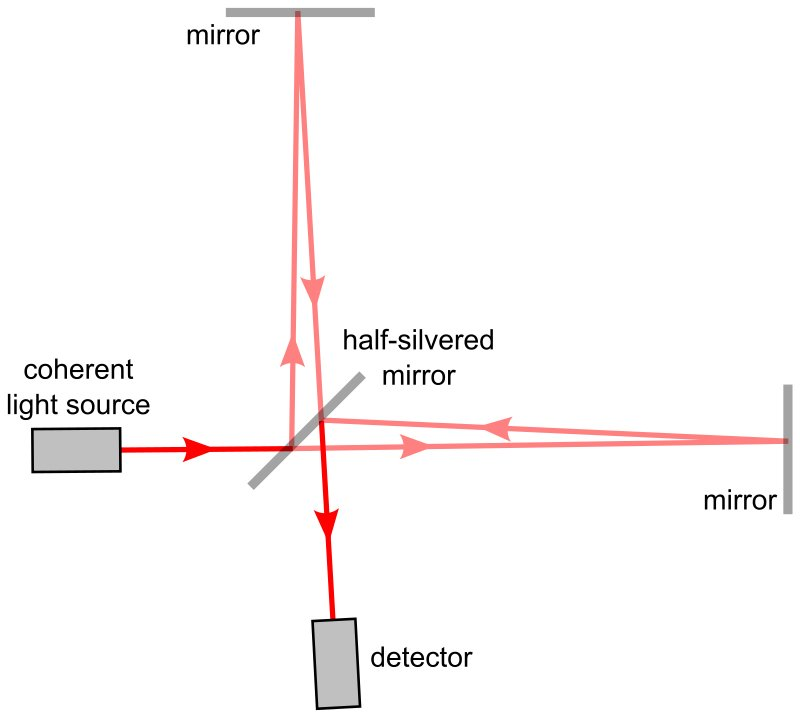
\includegraphics[width=0.9\linewidth]{Interferometer}
        \center
        \caption{By varing the optical path length of the rays you see constructive or destructive interference on the
        detector. This depends on the wavelength of the ligth, which enables you to measure it.
        Graphic from~\cite{imageMichelsonInterferometerWiki}}
        \label{fig:Interferometer}
    \end{figure}
    
%    As the second approach we use an interferometer.
%    The emitted light is split by a fiberboard as semi-transparent mirror in two perpendicular rays.
%    They are then reflected by two metal sheets and reunited again by the fiberboard. 
%    The resulting ray interferes constructively or destructively depending on the difference between the two optical paths .
%    We move the position of one mirror to change the optical path.
%    After seeing 15 maxima and minima on the detector we read the changed
%    path length.
%    With our setup we have determined the wavelength as:
    
    Die Eigenschaft, dass zwei kohärente Wellen interferieren, kann auch mit Hilfe eines Michelson-Interferometer
    nachgewiesen werden.
    In dem Michelson-Interferometer wird der ausgesendete Lichtstrahl zu nächst von einem halb-durchlässigen
    Spiegel in zwei senkrecht zueinander liegende Strahlen aufgespalten.
    Wir nutzen eine Hartfaserplatte.
    Diese ist semi-transparent für Mikrowellen.
    Die beiden aufgespalteten Lichtstrahlen werden von jeweils einem Spiegel zurück reflektiert auf den
    halb-durchlässigen Spiegel.
    Dieser führt die Strahlen wieder zusammen.
    Die beiden Strahlen interferieren dann mit einander.
    Sie interferieren entweder konstruktiv wenn der Gangunterschied der beiden Weglängen ein vielfaches der Wellenlänge ist:
    \begin{align*}
        \delta s = n \lambda & n \in \mathds{N}
    \end{align*}
    oder destruktiv falls gilt:
    \begin{align*}
        \delta s = (n + \frac{1}{2}) \lambda & n \in \mathds{N}
    \end{align*}
    
    Dieses Phänomen kann auch dazu genutzt werden, um die Wellenlänge zu bestimmen.
    Wir verwenden hierzu den oben beschriebenen Aufbau, wie er auch in Abbildung~\ref{fig:Interferometer}
    dargestellt ist.
    Auch hier variieren wir die Position des ersten Spiegels, bis wir ein Minima finden.
    Wir verschieben ihn nun nach außen und zählen wie viele Knoten der Empfänger detektiert.
    Nach dem wir $\NodeCountInterferometer$ Knoten durchlaufen sind, bestimmen wir wieder den
    Wegunterschied.
    Hieraus ergibt sich die Wellenlänge:
    
    \begin{align*}
        \lambda = \InterferometerWaveLength
    \end{align*}
    
    Der Fehler bestimmt sich auch hier aus den Positionsfehlern der Minima, welcher
    auf $\sigma_s = \PosErrorInterferometer$ geschätzt wird.s
    
    \section{Polarisation}

    \figPolarisation{Transmitted intensity through a polarisation filter.
    Though the shape of the curve fits, there is a strong deviation from the theory by Malus ~\eqref{eq:cos4}}
    
%    The Gunn diode with the horn antenna in our setup emits vertical polarized light.
%    Also the receiver detects in default configuration only vertical polarized light.
%    This can be easily shown by rotating the receiver about $ 90\degree$.
%    Now no signal is being detected.
%    If you then insert a linear polarisation filter in a $ 45\degree$ angle you will detect a signal.
%    This follows because the vertical polarized E-field is projected on the polarisation filter.
%    For the polarisation filter a simple metal grid was used with 22 lattice bars.
%
%    As a quantitative assertion we arranged the receiver and emitter in vertical position and rotated the polarisation
%    filter in an $ 180\degree $-arc and measured the angle-intensity distribution.
%    Following Malus's law~\cite{gerth} the intensity after the filter is:
    
    Elektromagnetische Wellen sind keine skalaren Wellen, sonder sie besitzen eine Polarisation.
    Dies liegt daran, dass sowohl das elektrische als auch das Magnetfeld Vektorfelder sind.
    Das E- bzw.\ B-Feld steht bei einer elektromagnetischen Welle senkrecht zur Ausbreitungsrichtung.
    Dadurch erhält die Welle eine Ausrichtung, die Polarisation.
    
    Zunächst wollen wir die Polarisation qualitativ nachweisen.
    Die Gunn-Diode emittiert und der Empfänger detektiert ausschließlich linear polarisiertes Licht.
    Dies kann überprüft werden in dem man Transmitter und Empfänger zunächst in Normallage bringt.
    Man detektiert ein Signal.
    Dreht man nun den Empfänger um $90^\circ$ dann misst man kein Signal.
    Dies liegt daran, der Transmitter emittiert v-polarisiertes Licht aber der Empfänger detektiert in
    dieser Ausrichtung nur h-polarisiertes Licht.
    Bringt man nun einen linearen Polfilter im $45^\circ$-Winkel zwischen Sender und Empfänger, dann wird
    wieder ein Signal detektiert.
    Dies liegt daran, dass das emittierte v-polarisierte Licht zur Hälfte auf den Winkel des Polfilters
    projiziert. 
    Vom durchkommenden Licht wird dann wieder die Hälfte auf den Winkel des Emitters projiziert.
    Es wird also ein Viertel der Ausgangsintensität detektiert.
    
    Diese qualitativen Eigenschaften können auch quantitativ untersucht werden.
    Hierzu bringen wir Sender und Empfänger in Normalstellung.
    Dazwischen positionieren wir nun den Polfilter.
    Er ist ein Metalgitter mit 10 Stäben.
    Der Polfilter wird nun von $-90^\circ$ bis $+90^\circ$ gedreht und es wird das jeweilig detektierte Signal
    abhängig vom Winkel gemessen.
    
    Die Intensität nach einem Polfilter abhängig vom Winkel ist gegeben durch das Gesetzt von Malus:
    
    \begin{align}
        I = I_0 \cos^2(\phi)
    \end{align}
%    Since the metal grid and the receiver act as two polarisation filter our signal should follow the formula:
    
    Da das Metalgitter und der Empfänger als zwei Polfilter fungieren, gilt für uns die folgende Formel:
    
    \begin{align}
        \label{eq:cos4}
        I = I_0 \cos^4( \phi )
    \end{align}
    
%    If we compare the theoretical function to the measured data as in ~\ref{fig:Polarisation} we see a strong deviation.
%    Multiple factors could be responsible for this result.
%    Firstly the polarisation filter used, is a lattice consisting of 22 metal bars. 
%    The relatively low count of bars makes it not an ideal linear polarisation filter.
%    Furthermore signal loss over the distance may cause the deviation.
%    Lastly it could be because of the cutoff from the receiver.
%    Maybe too weak signals are being cutoff and so the curve is deformed.
%    To verify these hypotheses more measurements are required.
    
    Die Daten sind in Abbildung~\ref{fig:Polarisation} eingetragen zusammen mit dem theoretisch zu erwarteten
    Verlauf nach Malus, wobei dieser auf das Maximum des Signals normiert ist.
    Wie in der Abbildung zu erkennen gibt es eine starke Abweichung zwischen theoretischen und tatsächlichen
    Verlauf.
    Dies liegt daran, dass das Signal des Empfängers nicht proportional zur Intensität ist.
    D.h.\ wir können den Zusammenhang nicht quantitativ bestätigen.
    Dennoch lässt sich in der Kurve zumindest die erwartete Form des theoretischen Verlaufs erkennen.
    Dies lässt die Richtigkeit des Gesetzes von Malus vermuten.
    
    \section{Frustrierte Totalreflexion und Tunnel-Effekt}
    
    \begin{figure}[htbp]
        \includegraphics[width=0.9\linewidth]{setup-total-reflection}
        \centering
        \caption{Experimental setup for showing total reflection and tunnel effect.
        In the gap between the the double prism a evanescent wave is formed.
        The itensity declines exponentaly according to equation ~\eqref{eq:ExpTransDecline}}
        \label{fig:SetupTotalReflection}
    \end{figure}

    \figTotalReflection{We measure the transmitted and reflected signal at a double prism.
    The transmitted signal declines exponentially. This can be explained by the tunnel effect.}
    
%    An important property of light which we were able to show, is total reflection and evanescent waves.
%    For the experiment we emitted microwaves on a paraffin wax prism. 
%    On the $45\degree$ paraffin-air boundary the rays are totally reflected and we detect them in an $90\degree$ rotated
%    angle. 
%    After the paraffin-air boundary an evanescent wave is formed.
%    Its intensity declines exponentiall
    Ein weiteres wichtiges Phänomen, welches nur mit der Welleneigenschaft erklärt werden kann, ist das
    der frustrierten Totalreflexion.
    Laut geometrischer Optik gilt: trifft eine Lichtstrahl auf einen Übergang vom optisch dichteren zum optisch dünneren Medium 
    $n_1 > n_2$ unter einem genügend großem Winkel $\Theta$ dann wird der Lichtstrahl total reflektiert.
    Der Auftreffwinkel muss größer als der Grenzwinkel sein $\Theta \geq \Theta_g$.
    Für diesen gilt:
    \begin{align*}
        \sin(\Theta_g) = \frac{n_2}{n_1}
    \end{align*}
    
    Wenn man diesen Effekt nun Wellen-theoretisch beschreibt, dann stellt sich heraus, hinter der Grenzfläche
    bildet sich eine evaneszente Welle aus.
    Diese transportiert keine Energie.
    Die Intensität fällt exponentiell ab:
    \begin{align}
        \label{eq:ExpTransDecline}
        I_{trans} = I_0 e^{\frac{-2x}{s}} 
    \end{align}
%    Here $x$ is the perpendicular distance and $s$ is the declination rate which depends on the wavelength, 
%    the angle of reflection and the refractive index.
%    Because of energy conservation, the reflected intensity is:
    Wobei $x$ der senkrechte Abstand zur Oberfläche ist und $s$ ein Maß für die Eindringtiefe.
    Diese hängt von der Wellenlänge ab, den Auftreffwinkel $\Theta$ und den Brechungsindex $n_1$ ab:
    \begin{align}
        s = \frac{\lambda}{2 \pi \sqrt {n_1^2 \sin^2(\Theta) - 1}}
    \end{align}
    
    Wir erzeugen die evaneszente Welle indem wir das Signal des Senders zunächst mit Hilfe der
    Wachslinse zu Parallelstrahlen bündeln.
    Diese werden auf ein Paraffinprisma gesendet, sodass die Strahlen an der $45^{\circ}$ Seite
    total reflektiert werden.
    Die reflektierten Strahlen werden dann vom Empfänger in Stellung B detektiert, wie in der
    Abbildung~\ref{fig:SetupTotalReflection} gezeigt.
    
    Bringt man nun ein zweites Prisma im Abstand $x$ hinter das erste Prisma, dann kann ein Teil der Welle
    `durch tunneln'.
    Die transmittierte Welle wird vom Detektor in Stellung A aufgezeichnet.
    Die Intensität der transmittierten Welle fällt exponentiell zum Abstand nach Gleichung~\eqref{eq:ExpTransDecline}.
    Die Intensität der reflektierten Welle muss dann wegen Energieerhaltung dem folgenden Verlauf folgen:
    
    \begin{align*}
        I_{ref} = I_0 (1 - e^{\frac{-2x}{s}})
    \end{align*}
    
%    You can detect the evanescent wave by a adding a second prism after the $ 45\degree$ boundary parallel to the first one
%    in the distance $x$.
%    Now analogous to the quantenmechanical tunnel effect\cite{gerth} the light can propagate through the air gap and a signal can be
%    detected.
%    We have measured the reflected and transmitted microwaves for different gap sizes $x$ and then applied an exponential 
%    fit as you can see in~\ref{fig:TotalReflection}
    
    Wir haben für verschiedene Abstände $x$ das reflektierte und transmittierte Signal gemessen.
    Die Daten sind in Abbildung~\ref{fig:TotalReflection}.
    Ferner haben wir eine Exponentialfunktion an die Daten angepasst.
    Die Daten scheinen gut einem exponentiellen Verlauf zu folgen.
    Der Fit hat ein angepasstes R-Quadrat von:
    \begin{align*}
        \bar{R}^2 = \TransmittedExpModelAdjustedRSquared
    \end{align*}
    Das die Spannung so gut einem exponentiellen Verlauf folgt ist von vorne herein nicht gegeben, da die
    Spannung nicht proportional zur Intensität ist.
    Es lässt aber vermuten, dass eventuell ein polynomieller Zusammenhang besteht:
    \begin{align*}
        U \propto I^{\alpha}
    \end{align*}
    
    
    \section{Bragg-Reflexion}
%    If you have monochromatic waves with a wavelength around the atomic scale (x-ray, neutrons or electrons) you can
%    determine the lattice constant $d$ of a cubic crystal via bragg diffraction. 
%    In Bragg's model the crystal is a set of discrete planes, where waves are being reflected.
%    If the waves have the correct wavelengths and hit the planes in the correct angle, the reflected waves interfere 
%    constructively and you see a bragg peak as a result~\cite{gerth}.
%    
%    The crystal planes can be indexed via the parameters $(h,\,k,\,l)$ .
    
    Eine wichtige Anwendungen der oben demonstrierten Reflexions- und Interferenzeigenschaften des Lichts ist das
    der Bragg-Reflexion.
    Hiermit lassen sich die Gitterkonstanten von Kristallstrukturen bestimmen, sofern man Wellen mit der
    entsprechenden Wellen länge zur Verfügung hat.
    Für die Untersuchung von Atomgittern benötigt man Wellenlänge auf der {\AA}ngström-skala (Röntgenstrahlung,
    Neutronen, Elektronen).
    
    Zur Demonstration der Bragg-Reflexion nutzen wir ein makroskopisches Kristallmodel.
    Das Model ist ein Styropor-Würfel indem 5x5x4 $10\,\mathrm{mm}$ große Metalkugeln eingebettet sind.
    Wir können die Gitterkonstanten von verschiedene Ebenen bestimmen.
    Die Ebenen werden mit den Miller-Indizes $(h,\,k,\,l)$ durch nummeriert, wie
    in Abbildung~\ref{fig:BraggPlanesIndices} dargestellt.
    
    \begin{figure}[htbp] % TODO Pasco Picture
        \centering
        \begin{subfigure}{0.49\linewidth}
            \centering
            \includegraphics[width = \linewidth]{Miller_Indizes_Ebenen_100}
        \end{subfigure}
        \begin{subfigure}{0.49\linewidth}
            \centering
            \includegraphics[width = \linewidth]{Miller_Indizes_Ebenen_110}
        \end{subfigure}
        \caption{Bragg-planes for a cubic crystal model with indices $(h,\,k,\,l)$.
        Images from ~\cite{miller}}
        \label{fig:BraggPlanesIndices}
    \end{figure}

    \figBraggReflectionOneZeroZero{Bragg diffraction on the 100-plane of a cubic lattice model.
    A peak was detected at the first bragg-maxima}
    \figBraggReflectionOneOneZero{Bragg diffraction on the 110-plane of a cubic lattice model.
    Here the bragg-peak occurs at a greater angle compared to the 100-palne}

    Damit die Bragg-Bedinung erfüllt ist muss zunächst der Winkel der einlaufenden Welle $\Theta$ gleich der 
    reflektierten Welle sein.
    In unserem Experiment realisieren wir dies, indem wir das Kristallmodel auf einen Drehtisch montieren.
    Dieser wird dann um den Winkel $\Theta$ gedreht.
    Der Empfänger wird auf einen weiteren Dreharm montiert.
    Dieser wird um den Winkel $2 \Theta$ gedreht.
    Der Abstand zwischen Kristall und empfänger ist ca.\ $70 \, \mathrm{cm}$.
    
    Ferner damit die Bragg-Reflexion gut funktioniert, benötigen wir Parallelstrahlen.
    Wir nutzen hierzu die Wachslinse indem wir den Transmitter auf den Brennpunkt der Linse stellen.
    
%    For the angle $\Theta$, for which a peak occurs, the following relation applies:
    Die einlaufenden Lichtstrahlen werden an den verschiedenen Ebenen reflektiert.
    Es kommt zu konstruktiver Interferenz zwischen den reflektierten Lichtstrahlen, falls die Bragg-Bedingung erfüllt
    ist:
    \begin{align}
        \label{eq:BraggAngle}
        \frac{d}{\sqrt{h^2+k^2+l^2}} = n \frac{\lambda}{2 \sin(\Theta)} & n \in \mathds{N}
    \end{align}
    
    Hier ist $d$ die Gitterkonstante, $\lambda$ die Wellenlänge des Lichts und $n$ ist das n-te Beugungsmaxima.
    In unseren Messungen sehen wir nur ein Bragg-Maximum, deshalb ist $n = 1$.
    
%    To demonstrate the principle, we use a basic crystal model, consisting of metal bars arranged in a grid structure.
%    For examining real crystals, it would require electromagnetic waves with much smaller wavelengths.
%    We realize the experiment by placing the emitter in the focal point of the wax lens, so the crystal is hit by
%    parallel light-rays.
%    The crystal model is then rotated about $\Theta$ and the detector about $2\Theta$, to actualize the Bragg condition.
%    
%    We have done two measurement-series: For the plane-orientation $(h=1,\,k=0,\,l=0)$ and for $(h=1,\,k=1,\,l=0)$.
%    As you can see in figure~\ref{fig:BraggReflectionOneZeroZero} and figure~\ref{fig:BraggReflectionOneOneZero}.
%    If we use equation~\eqref{eq:BraggAngle} to calculate the lattice constant from our measurement-series, we get:
    
    Wir haben die Messung für die $(h=1,\,k=0,\,l=0)$-Ebene und die $(h=1,\,k=1,\,l=0)$-Ebene durchgeführt.
    Die Messreihen sind in Abbildung~\ref{fig:BraggReflectionOneZeroZero} und Abbildung~\ref{fig:BraggReflectionOneOneZero}
    dargestellt.
    Aus den Abbildungen wurde die Lage der Maxima abgeschätzt.
    Der Fehler wurde auf Grund der graphischen Methode wurde der Fehler groß angesetzt $\sigma_{\Theta} = \BraggDiffractionErrorAngle$.
    Mit Gleichung~\ref{eq:BraggAngle} kann hieraus die Gitterkonstante $d$ berechnet werden:
    
    \begin{align*}
        d_{100} = \CristalconstantOneZeroZero \\
        d_{110} = \CristalconstantOneOneZero
    \end{align*}
    
    Die Werte stimmen innerhalb ihrer Fehler überein.
    Laut Anleitung ist die tatsächliche Gitterkonstante des Kristallmodels:
    \begin{align*}
        d = 3.8 \, \mathrm{cm}
    \end{align*}
    Die Werte stimmen nicht überein.
    Die Ungenauigkeit der Methode kann damit erklärt werden, dass das vom Kristall reflektierte Signal
    relativ schwach ist.
    Somit können unerwünschte Reflexionen an anderer Stelle das Signal stören.
    Ferner ist die Anzahl der Ebenen mit 5 sehr gering.
    Die Schärfe des Bragg-Peaks steigt mit der Anzahl der Ebenen.
    Trotzdem konnte das Prinzip der Bragg-Reflexion demonstriert werden.
    
    \section{Waveguide}
    
    Lastly we examined a simple waveguide for microwaves.
    We used a basic metal tube.
    The waves are being reflected in its interior and thus guided by the tube.
    We placed the emitter at one end of the tube and the receiver at the other.
    A signal is being detected.
    If you plug one end, no signal is being detected.
    This proves, the waves are guided inside of the tube and not on its surface.
    Also the tube preserves the polarisation of the emitted light.
    This was shown by simply rotating the receiver, since it only detects v-polarized light.

    \section{Summary}
    
    At first we tested our experimental setup.
    The Gunn diode has a gaussian angle-intensity distribution with a variance $fwdh = \AngleDispersionGaussFWHM$.
    To focus the microwaves we used a wax lens with a focal length $f = \FocalLength$.
    Then we used two approaches to measure the wavelength. 
    Via stationary waves we get a wavelength $\lambda = \StandingWavesWaveLength$.
    The michelson interferometer produces a similar result $\lambda = \InterferometerWaveLength $.
    We could show the polarization of the emitted light and at least qualitatively verify Malus' law. 
    The effect of total reflection and tunnel effect was demonstrated by using a double prism.
    The intensity of the evanescent waves declines exponentially.
    We used a crystal model to show the method of bragg diffraction.
    The lattice constant was determined to be $d_{100} = \CristalconstantOneZeroZero$.
    At last we used a metal tube as waveguide.
    We demonstrated qualitatively it preserves the polarisation of the guided light.
    
    
    %FF: Angabe der verwendeten Literatur mit Quellennachweis.
    \begin{thebibliography}{}    %so wird das Literaturverzeichnis erstellt
        \bibitem{instr} Physikalisches Grundpraktikum, Universitüt Würzburg, Modul C1, Versuch 42, Versuche mit Mikrowellen - Kristallinterferenzen mit Mikrowellen, 2021
        \bibitem{gerth} Meschede, Dieter, Gerthsen Physik, 25. Auflage, Springer-Verlag, Berlin, 2015
        \bibitem{codata} P. J. Mohr, D. B. Newell, and B. N. Taylor: \grqq CODATA
        recommended values of the fundamental physical constants: 2014\grqq , Rev. Mod. Phys.
        88, 035009 (2016))
        \bibitem{miller} \url{https://de.wikipedia.org/wiki/Datei:Miller_Indizes_Ebenen.png}, zuletzt aufgerufen am 14.09.2021
        \bibitem{pasco} Pasco Microwave Optics System (WA-9314C) Instruction Manual
        %\bibitem{missing} \url{https://en.wikipedia.org/wiki/Transverse_mode}, zuletzt aufgerufen am 8.10.2021
        \bibitem{imageMichelsonInterferometerWiki} \url{https://en.wikipedia.org/wiki/Michelson_interferometer#/media/File:Michelson_interferometer_with_labels.svg}, last visit 23.09.23
    \end{thebibliography}
    
\end{document}